\documentclass[10pt]{article}
\usepackage{amsmath}
\usepackage{amssymb}
\usepackage{setspace}
\usepackage{tasks}
\usepackage{graphicx}
\usepackage{float}
\usepackage{listings}
\usepackage[utf8]{inputenc}
\usepackage{amsfonts}
\usepackage{gensymb}
\usepackage{multicol}
\usepackage{tabularx}
\usepackage{tikz}
\usetikzlibrary{arrows,shapes,automata,petri,positioning,calc}
\usepackage{hyperref}
\usepackage[margin=1.0in]{geometry}

% Power functions
\newcommand{\myvec}[1]{\ensuremath{\begin{pmatrix}#1\end{pmatrix}}}
\let\vec\mathbf

\newcommand{\mydet}[1]{\ensuremath{\begin{vmatrix}#1\end{vmatrix}}}
\providecommand{\brak}[1]{\ensuremath{\left(#1\right)}}
\providecommand{\lbrak}[1]{\ensuremath{\left(#1\right.}}
\providecommand{\rbrak}[1]{\ensuremath{\left.#1\right)}}
\providecommand{\cbrak}[1]{\ensuremath{\left\{#1\right\}}}
\providecommand{\sbrak}[1]{\ensuremath{{}\left[#1\right]}}
\providecommand{\norm}[1]{\left\lVert#1\right\rVert}
\providecommand{\abs}[1]{\left\vert#1\right\vert}

\begin{document}
\section*{9$^{th}$ Maths - Chapter 7}
This is Problem-5 from Exercise 7.1

\begin{enumerate}
\item Line $l$ is the bisector of an angle $\angle{A}$ and $B$ is a point on line $l$. $BP = BQ$ are perpendiculars from $B$ to the arms of $\angle{A}$. 
\begin{enumerate}
\item $\triangle{APB} \cong \triangle{AQB}$
\item $BP = BQ$ or $B$ is equidistant from the arms of $\angle{A}$
\end{enumerate}
\end{enumerate}
\begin{figure}[H]
    \begin{center}
    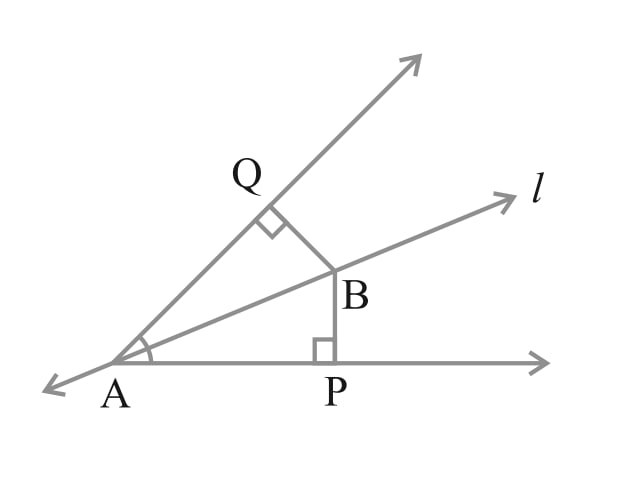
\includegraphics[width=80mm]{figs/QAPB.png}
    \caption{$l$ bisecting $\angle{A}$}
    \label{triangle BAQ  and BAP }   
\end{center}
\end{figure}
\textbf{Construction:}

The input parameters for the construction are shown in Table
\begin{center}
\begin{table}[h]
 \renewcommand{\arraystretch}{1.5}
 \centering
     \begin{tabular}{|c|c|p{6cm}|}
        \hline
        \textbf{Symbol} & \textbf{Value} & \textbf{Description} \\
        \hline
        $\theta$ & $30^\circ$ & $\angle BAQ = \angle BAP$ \\
        \hline
        $a$ & $7$ & Length of $AB$ \\
        \hline
        $c$ & $6$ & Length of $AQ$ \\
        \hline
        $\vec{e}_1$ & $\begin{pmatrix} 1 \\ 0 \end{pmatrix}$ & Basis vector \\
        \hline
    \end{tabular}

 \caption{ values and descriptions.}
 \label{tab:symbols}
\end{table}
\end{center}
	

Let $\vec{A} = \myvec{0\\0}$, $\vec{B} = a\vec{e_1}$, $\vec{Q} = \myvec{c\cos\theta\\c\sin\theta}$, and $\vec{P} = \myvec{c\cos\theta\\-c\sin\theta}$.

\section*{Solution:}
\textbf{Given:}

\begin{align}
\angle{BAQ} &= \angle{BAP} \quad \brak{\text{line \text{`$l$'} bisects $\angle{A}$}}\\
\angle{AQB} &= \angle{APB} \quad \brak{\text{Both angles are $90^{\degree}$}}
\end{align}
\textbf{To Prove:}
\begin{enumerate}
\item $\triangle{APB} \cong \triangle{AQB}$
\item $BP = BQ$ or $B$ is equidistant from the arms of $\angle{A}$
\end{enumerate}

\textbf{Proof:}
\begin{center}
In $\triangle{APB}$ and $\triangle{AQB}$
\end{center}
\begin{align}
\angle{BAQ} &= \angle{BAP} \quad \brak{\text{line \text{`$l$'} bisects $\angle{A}$}}\\
\angle{AQB} &= \angle{APB} \quad \brak{\text{Both angles are $90^{\degree}$}}\\
AB	 &= AB \quad \brak{\text{common side for both triangles}}
\end{align}
 Therefore, by Angle-Angle-Side (A-A-S) congruence rule, $\triangle{APB} \cong \triangle{AQB}$.\\
 Now we have to prove $BP$ = $BQ$
\begin{align}
\norm{\vec{B} - \vec{P}} & = \sqrt{\brak{\vec{B} - \vec{P}}^\top \brak{\vec{B} - \vec{P}}}\\
\brak{\vec{B} - \vec{P}} & = \myvec{7\\0} - \myvec{6\cos\theta\\-6\sin\theta} \implies \myvec{7-6\cos\theta\\-6\sin\theta} \implies \myvec{7-5.19\\ -3} \implies \myvec{1.81\\ -3}\\
\brak{\vec{B} - \vec{P}}^\top & = \myvec{7-6\cos\theta & -6\sin\theta} \implies \myvec{1.81 & -3}\\
\brak{\vec{B} - \vec{P}}^\top \brak{\vec{B} - \vec{P}} & = \myvec{1.81 & -3} \myvec{1.81\\ -3} \implies 12.27 \\
\norm{\vec{B} - \vec{P}} & = \sqrt{12.27} = 3.5\\
Similarly  Now,\norm{\vec{B} - \vec{Q}} & = \sqrt{\brak{\vec{B} - \vec{Q}}^\top \brak{\vec{B} - \vec{Q}}}\\
\brak{\vec{B} - \vec{Q}} & = \myvec{7\\0} - \myvec{6\cos\theta\\6\sin\theta} \implies \myvec{7-6\cos\theta\\6\sin\theta} \implies \myvec{7-5.19\\ 3} \implies \myvec{1.81\\ 3}\\
\brak{\vec{B} - \vec{Q}}^\top & = \myvec{7-6\cos\theta & 6\sin\theta} \implies \myvec{1.81 & 3}\\
\brak{\vec{B} - \vec{Q}}^\top \brak{(\vec{B} - \vec{Q}} & = \myvec{1.81 & 3} \myvec{1.81\\ 3} \implies 12.27 \\
\norm{\vec{B} - \vec{Q}} & = \sqrt{12.27} = 3.5\\
\norm{\vec{B} - \vec{P}} & = \norm{\vec{B} - \vec{Q}}
\end{align}
Therefore, $BP = BQ$ or $B$ is equidistant from the arms of $\angle{A}$ is proved
\begin{figure}[H]
    \begin{center}
    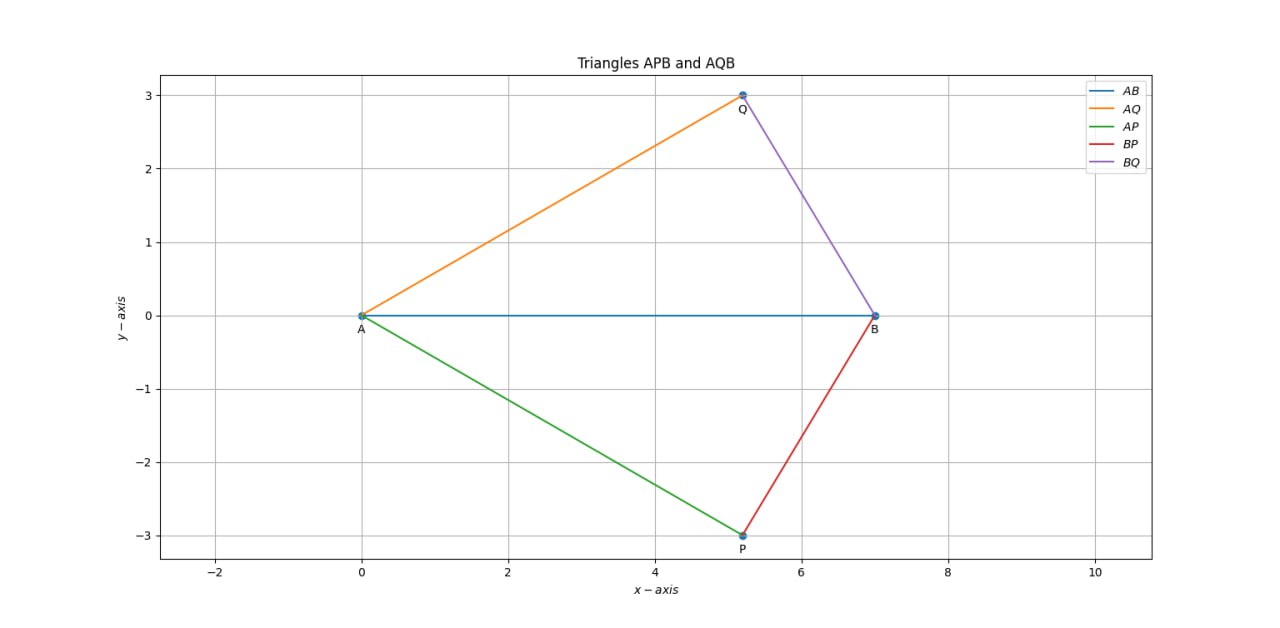
\includegraphics[width=\columnwidth]{figs/pythongraph.png}
    \caption{python graph plot}
    \label{triangle $BAQ$  and $BAP$ }   
    \end{center}
\end{figure}
\end{document}
